The first subsection explains the system's architecture in detail based on a \ac{UML} diagram. With this diagram, it is possible to show the component-based architecture and how the mentioned tools are combined for the different visualisations and concepts. The second subsection shows the transition manager in detail, which features the transition table mentioned in Chapter \ref{s:theoretical-contrib} on page \pageref{s:theoretical-contrib}.
As already mentioned in Chapter \ref{s:collaboration-statement} on page \pageref{s:collaboration-statement}, \citeauthor{Wanko2016} is researching on a related topic of this thesis. The practical part of his thesis and the one of this thesis are implemented in the same system. Therefore, the actual application has a lot more features and options than described in this section.

\subsubsection{Application Architecture}
Figure \ref{fig:uml-practical-approach} on page \pageref{fig:uml-practical-approach} gives an overview of the architecture in the form of a class diagram. However, the diagram shown and discussed in the master-thesis of \citeauthor{Wanko2016} looks quite different, although it is based on the same system. This is due to the relatively big system architecture and the different scopes of both theses \iacite{Wanko2016}. Showing and discussing all available classes, features and options for the application would go beyond the scope of this thesis. The following list briefly discusses the most important classes and their purposes:

%TC:ignore
\begin{figure}[!htb]
\centering
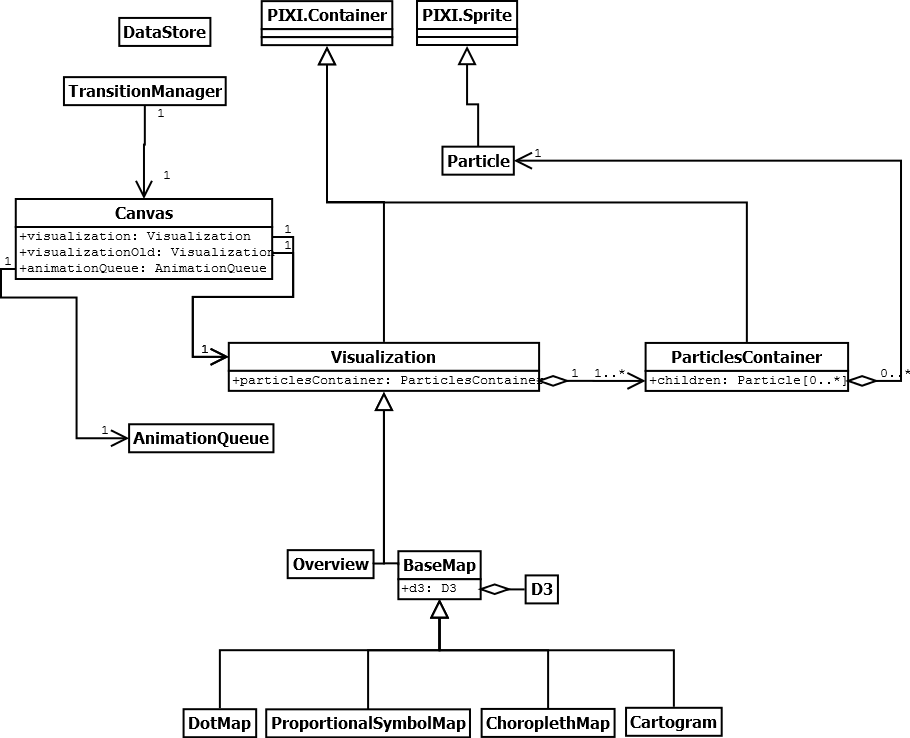
\includegraphics[width=0.8\textwidth,keepaspectratio]{images/results/dia.png}
\caption[
    Overview of the application architecture in the form of a class diagram.
]{Overview of the application architecture in the form of a class diagram.}
\label{fig:uml-practical-approach}
\end{figure}
%TC:endignore

\begin{description}
\item[DataStore] \hfill \\
An object of the DataStore-class is used to load the SuperStore-Sale dataset. In addition to initally loading it, it also parses and analyses the dataset. Each attribute of the dataset gets classified in order to handle the attributes correctly later on. For the sake of convenience, four different classification types were used: numeric, date, nominal and unknown.

\item[PIXI.Container] \hfill \\
\ac{Pixi} features functionalities like container classes. \textit{PIXI.Container} is such a class and can be used to put objects in it, and scale or move those objects according to the base-canvas.

\item[AnimationQueue] \hfill \\
If an animation is assigned to particles, it is stored in the \textit{AnimationQueue}. This allows to create multiple canvas-based animations and process them sequentially.

\item[Canvas] \hfill \\
This class is one of the main classes inside the application. It is needed to not compare it with an HTML-Canvas object. It is responsible for creating the base-canvas of the web-application. Furthermore, it is used to change and update the visual appearance if any interaction happens. A key part of the canvas class is the render function shown in Listing \ref{lst:canvas-render} on page \pageref{lst:canvas-render}. It starts off with calling the same function again as soon as possible. The caller-function \textit{requestAnimationFrame} ensures, that the next frame will only be shown if enough resources of the browser are available. Afterwards, all particles and visualisations are animated if something changed. The last line of the listing shows the \ac{Pixi}-renderer. Listing \ref{lst:canvas-autodecet-renderer} on page \pageref{lst:canvas-autodecet-renderer} shows its creation. It features the main canvas-size, background transparency and antialiasing. The renderer provides considerably more options which are not used.

%TC:ignore
\begin{lstlisting}[language=JavaScript, caption={Render function of the canvas class.}, label={lst:canvas-render}]
    render() {
      this.requestFrameID = requestAnimationFrame(this.render.bind(this));

      let areParticlesAnimating = this.particlesContainer.nextStep();
      let isNewVisualizationAnimating = this.visualization.nextStep();
      let isOldVisualizationAnimating = this.visualizationOld ? this.visualizationOld.nextStep() : false;

      if (!areParticlesAnimating && !isOldVisualizationAnimating &&
        !isNewVisualizationAnimating && this.animationQueue.length > 0) {

        this.animationQueue.pop()();
        this.particlesContainer.startAnimation();
        this.visualization.startAnimation();
        if (this.visualizationOld){
            this.visualizationOld.startAnimation();
        }
      }
      this.renderer.render(this.stage);
    }
\end{lstlisting}

\begin{lstlisting}[language=JavaScript, caption={Pixi's autodetect-renderer.}, label={lst:canvas-autodecet-renderer}]
    this.renderer = PIXI.autoDetectRenderer(this.width, this.height, {
        transparent: true,
        clearBeforeRender: true,
        antialias: true
    });
    document.body.appendChild(this.renderer.view);
\end{lstlisting}
%TC:endignore

\item[Visualization] \hfill \\
This class is the starting point and the parent class for all other types of visualisations. It stores a reference to the \textit{ParticleContainer} and provides functionality to move, scale or change visualisations.

\item[Overview] \hfill \\
Creating an instance of \textit{Overview} shows all data items as unit-based grid.

\item[D3] \hfill \\
This class is mainly used to wrap all functionality of the \ac{D3} library. It features functions like initialising the base-map as a \ac{SVG} and loading the needed TopoJSON data accordingly. \ac{D3} offers multiple projections for GeoJSON data. Listing \ref{lst:d3-map-init} on page \pageref{lst:d3-map-init} shows a part of the map initialisation with the projection used. The used projection is an extension of an Albers equal-area projection discussed in Chapter \ref{s:map-projections} on page \pageref{s:albers-equal-area-projection}. It is a United-States-centric composite projection. The lower forty-eight states of America are projected using the default Albers-equal-area projection. However, Alaska and Hawaii use a separate conic equal-area projection. The scale of Alaska is furthermore diminished. It is projected at $0.35\times$ its true relative area. The scale and translation of the map are set to use the available window space and center the map on the screen.

%TC:ignore
\begin{lstlisting}[language=JavaScript, caption={Map initialisation with a map projection, scale, and translation.}, label={lst:d3-map-init}]
    this.projection = this._d3.geo.albersUsa()
        .scale(width)
        .translate([this.width / 2, this.height / 2]);
\end{lstlisting}
%TC:endignore

Another key part of this class is featured in Listing \ref{lst:d3-topojson} on page \pageref{lst:d3-topojson}. It shows how TopoJSON is used on the client. The filter function passed to the first \textit{TopoJSON.mesh}-function specifies that only internal state borders should be used. Thus, coastlines will not be drawn to retain detail around small islands and inlets. The filter function passed to the second \textit{TopoJSON.mesh}-function extends the first one by only showing each county boundary once. Thus, if two counties share the same border, it is only drawn once later on.

%TC:ignore
\begin{lstlisting}[language=JavaScript, caption={TopoJSON usage on the client with the adaption of merging all geographic information.}, label={lst:d3-topojson}]
    this.data.topojson.states = topojson.mesh(
        this.data.us,
        this.data.us.objects.states,
        (a, b) => {
            return a !== b;
        }
    );

    this.data.topojson.counties = topojson.mesh(
        this.data.us,
        this.data.us.objects.counties,
        (a, b) => {
            return (
                a !== b &&
                !(this.getCountyIdentifier(a) / 1000 ^ this.getCountyIdentifier(b) / 1000)
            );
        }
    );
\end{lstlisting}
%TC:endignore

Another important aspect of the \ac{D3} class is the \textit{calculateCentroids}-function shown in Listing \ref{lst:d3-calculate-centroids} on page \pageref{lst:d3-calculate-centroids}. It pre-calculates a look-up dictionary for the given level of detail for each data item. Thus, it provides a huge performance boost when finding out the centroid of a unit later on.

%TC:ignore
\begin{lstlisting}[language=JavaScript, caption={Calculate a look-up dictionary for all data items depending on the level of detail.}, label={lst:d3-calculate-centroids}]
    calculateCentroids(levelOfDetail){
        const boundaries = this._topojson.feature(
            this.data.us,
            this.data.us.objects[levelOfDetail]
        ).features;

        this.centroids[levelOfDetail] = {};
        for(let boundary of boundaries){
            this.centroids[levelOfDetail][boundary.id] = this.path.centroid(boundary);
        }
    }
\end{lstlisting}
%TC:endignore

Furthermore, this class exposes two mandatory functions used to create aggregated thematic maps. Listing \ref{lst:d3-scales} on page \pageref{lst:d3-scales} features the scaling methods used in the application. The \textit{symbolScale}-method is based on a power scale with the input domain ranging from $0$ to $1000000$ and the output domain ranging from $0$ to $10$. The default exponent is $0.5$. If an input value exceeds the given domain, it is scaled and interpolated automatically respectively to the scale and a higher output range.
The colour scale is based on a quantise scale which are similar to linear scales, except they use a discrete rather than continuous range. The continuous input domain is divided into uniform segments based on the number of values in the output range. The output range is not shown in the listing because it depends on the chosen colour scheme. However, each scheme is represented by an array of 9 different colours. Thus, each range value can be expressed as a quantised linear function of the domain value.
Both scaling methods do not change their input domain throughout the application, even when changing the level of detail. The only change on a scale is the output colour of the \textit{colorScale}-method. As a result, the symbol size and colour used are not linked to the level of detail, but rather map the a particular input value always to the same output value.

%TC:ignore
\begin{lstlisting}[language=JavaScript, caption={Symbol-scale and colour-scale used for aggregated thematic maps.}, label={lst:d3-scales}]
    this.symbolScale = this._d3.scale.sqrt()
    .domain([0, 1e6])
    .range([0, 10]);

    this.colorScale = this._d3.scale.quantize()
    .domain([0, 1000]);
\end{lstlisting}
%TC:endignore

\item[BaseMap] \hfill \\
This is the second class inheriting from the \textit{Visualization} class. It features a single object of the \ac{D3} class. Therefore, it is possible that all deriving classes share the same object of \ac{D3} and thus, all its features and settings. Changing the level of detail of the \textit{BaseMap} will affect the map initialised in \textit{\ac{D3}} and hence, all deriving classes are using the same base-map again. This main purpose of this class is the Singleton object of \ac{D3} for all children.
The decision if and how the upcoming map should be animated or not handles each subclass on its own. All subclasses based on aggregation are implemented and animated with \ac{D3}. Therefore, the dot map is slightly different than these in the terms of structure and usage. Furthermore, all thematic maps based on aggregation are implemented with the method of using a static file containing all information. However, the aggregated values could also be calculated dynamically every time.

\item[DotMap] \hfill \\
The \textit{DotMap} class is the first one to show data on the base-map. It does not use the \ac{DOM} to create the dots (also called particles) on the map. It uses the already existing particles from the particle container inherited from the \textit{Visualization} class. Key part of this class is the initial position of all particles because the dot map is used as an overview of the used data. Listing \ref{lst:dot-draw-animated} on page \pageref{lst:dot-draw-animated} shows the initial placement. Each particle has geographical information denoted as \textit{particle.data.Longitude} and \textit{particle.data.Latitude} which is projected onto the map. The subsequent code saves the projection on the particle object and sets its size and position.

%TC:ignore
\begin{lstlisting}[language=JavaScript, caption={Particles on a dot map getting animated.}, label={lst:dot-draw-animated}]
    for(let particle of this.particles){
        point = [particle.data.Longitude, particle.data.Latitude];
        point = this.baseMap.projection(point);
        particle.coords = point;
        particle
        .setPosition(
            particle.coords[0]-(this.size/2),
            particle.coords[1]-(this.size/2)
        )
        .setSize(
            this.size,
            this.size
        );
    }

\end{lstlisting}
%TC:endignore

\item[ProportionalSymbolMap] \hfill \\
The implemented proportional symbol map is a multivariate classed proportional symbol map. The symbol size is scaled with the herein before mentioned symbol scale method. The population of the enumeration unit is the input domain of the method and therefore its symbol size. The second attribute is mapped with colour onto each symbol. The amount of orders of each enumeration unit is used. The amount is classified in a range of $9$ possible classes, where each class is represented by a colour of a sequential colour scale.
Drawing the multivariate classed proportional symbols is done by using \ac{D3}. First of all, it does not use the SuperStore-Sale file as a basis, and instead uses the preprocessed TopoJSON file. The class exposes functions like \textit{initSymbols}, \textit{colorSymbol}, \textit{scaleSymbols}, and so forth. Each function handles a single concern offering the best possible flexibility to create animated transitions to different kinds of visualisations.

\item[ChoroplethMap] \hfill \\
The implementation of this type of thematic map is a univariate classified choropleth map, where each coloured area represents the amount of orders.

\item[Cartogram] \hfill \\
The web-application implements a specific type of cartogram: a pseudo Demers cartogram. A true Demers cartogram would need links between adjacent features. However, the type of cartogram implemented tries to preserve locality instead of connectedness. Furthermore, it uses circles instead of squares. This allows to create an animated transition from proportional symbols to a cartogram by applying a force with some kind of gravity without the need to change the symbol.
Preserving locality is done by placing each circle as close as possible to its origin without overlapping. In order to deliver this kind of information to the user, a collision detection with gravity is used to animate the position of each circle. Listing \ref{lst:cartogram-part-tick} on page \pageref{lst:cartogram-part-tick} shows a small part of the force directed layout. The \textit{tick}-method can be compared to the before mentioned \textit{render}-method of the canvas class. It executes every frame if possible and applies collision detection and gravity to every symbol. \textit{gravity}-method is a key part is this concept. The attributes \textit{x0} and \textit{y0} represent the origin of each symbol whereas \textit{x} and \textit{y} are the current coordinates changed by the collision function. Thus, the gravity function ensures, that the symbols are as close to their location as possible.

%TC:ignore
\begin{lstlisting}[language=JavaScript, caption={A small part of the draw-function of the pseudo Demers Cartogramm-class}, label={lst:cartogram-part-tick}]
    tick(gravity) {
        this[this.id]
        .each(this.gravity(gravity))
        .each(this.collide(0.25))
        .attr("cx", d => { return d.x; })
        .attr("cy", d => { return d.y; });
    }

    gravity(k) {
        return d => {
            d.x += (d.x0 - d.x) * k;
            d.y += (d.y0 - d.y) * k;
        };
    }
\end{lstlisting}
%TC:endignore

\item[ParticlesContainer] \hfill \\
This container contains all particles and ensures, that they are animated in the desired order. Furthermore, it controls the speed of each animated particle.

\item[Particle] \hfill \\
A particle inherits the functionality of \textit{PIXI.Sprite} and contains information about its position, alpha value, and the data it represents. It exposes methods to draw a particle onto the map and to animate it.

\item[TransitionManager] \hfill \\
If the type of visualisation changes, an instance of this class gets called. It handles all animations concerning the transition. The exposed \textit{animate}-function needs two parameters as strings: the type of the current visualisation and the type of the upcoming one. With this information, it is possible to handle each transition separately. Section \ref{s:animated-transitions-implemented} on page \pageref{s:animated-transitions-implemented} discusses the implemented and animated transitoins in detail.
\end{description}

Another aspect of all thematic maps based on aggregation is the stored reference of the data shown (the allocation of \textit{this[this.id] = \ldots}). This reference is used to determine if the data on the map needs to be updated and redrawn or not.
